%%%%%%%%%%%%%%%%%%%%%%%%%%%%%%%%%%%%%%%%%%%%%%%%%%%%%%%%%%%%%%%%%%
%%%%%%%% ICML 2015 EXAMPLE LATEX SUBMISSION FILE %%%%%%%%%%%%%%%%%
%%%%%%%%%%%%%%%%%%%%%%%%%%%%%%%%%%%%%%%%%%%%%%%%%%%%%%%%%%%%%%%%%%

% Use the following line _only_ if you're still using LaTeX 2.09.
%\documentstyle[icml2015,epsf,natbib]{article}
% If you rely on Latex2e packages, like most moden people use this:
\documentclass[10pt]{article}

% use Times
\usepackage{times}
% For figures
\usepackage{graphicx} % more modern
%\usepackage{epsfig} % less modern
\usepackage{float}

% For citations
\usepackage{natbib}

% For algorithms
\usepackage{algorithm}
\usepackage{algorithmic}
\usepackage{bm}
\usepackage{amssymb,amsmath}


% As of 2011, we use the hyperref package to produce hyperlinks in the
% resulting PDF.  If this breaks your system, please commend out the
% following usepackage line and replace \usepackage{icml2015} with
% \usepackage[nohyperref]{icml2015} above.
\usepackage{hyperref}

% Packages hyperref and algorithmic misbehave sometimes.  We can fix
% this with the following command.
\newcommand{\theHalgorithm}{\arabic{algorithm}}

% Employ the following version of the ``usepackage'' statement for
% submitting the draft version of the paper for review.  This will set
% the note in the first column to ``Under review.  Do not distribute.''
\usepackage[accepted]{icml2015}
\usepackage{amsmath}
\usepackage{amsmath}
\usepackage{amsfonts}
\usepackage{amssymb}

\usepackage{todonotes}

\usepackage{amsbsy}

% Employ this version of the ``usepackage'' statement after the paper has
% been accepted, when creating the final version.  This will set the
% note in the first column to ``Proceedings of the...''
%\usepackage[accepted]{icml2015}


% The \icmltitle you define below is probably too long as a header.
% Therefore, a short form for the running title is supplied here:

% Saving space by deleting running title (does this actually save space?)
%\icmltitlerunning{Submission and Formatting Instructions for ICML 2015}

\begin{document} 

\twocolumn[

% Saving space by deleting title
%\icmltitle{Submission and Formatting Instructions for \\ 
%           International Conference on Machine Learning (ICML 2015)}

% It is OKAY to include author information, even for blind
% submissions: the style file will automatically remove it for you
% unless you've provided the [accepted] option to the icml2015
% package.


% You may provide any keywords that you 
% find helpful for describing your paper; these are used to populate 
% the "keywords" metadata in the PDF but will not be shown in the document
\icmlkeywords{6.867, machine learning}

\vskip 0.3in
]

% Saving space by deleting abstract
%\begin{abstract} 
%The purpose of this document is to provide both the basic paper template and
%submission guidelines.
%\end{abstract} 

\section{Logistic Regression}



We used our gradient descent code from Homework 1 to solve this problem. In particular we supplied the optimizer with analytic gradients. If we define $\tilde{x}$ to be $[1,x]^T$ then the gradient of the regularized NLL objective can be written as
%
%
\begin{equation}
\frac{\partial E_{LR}(w)}{\partial w} = \sum_i -y^{(i)} \tilde{x}^{(i)} \frac{\exp(-y^{(i)}(\tilde{x}^{(i)}w + w_0))}{1 + \exp(-y^{(i)}(\tilde{x}^{(i)}w + w_0))}
\end{equation}
%
%
As was shown in lecture, the objective function for logistic regression is convex. Thus gradient descent should, with the appropriate step size and convergence threshold, converge to the global minimum. For almost all the subsequent optimizations we used a step size of $\eta = 1e-4$ and an initial guess of $w_{initial} = [0,0,0]$. A few optimizations (in particular those for very large $\lambda$) required a smaller step size, approximately $\eta = 1e-6$.

\subsection{$\lambda = 0$}

First we present the results for $\lambda = 0$ in Table \ref{lam_0}
\begin{table}[H]
\begin{tabular}{|c|c|}
\hline
dataset & misslassification rate \\ \hline
stdev1 train & $0$\\ \hline
stdev1 val & $0$\\ \hline
stdev2 train & $0.0925$\\ \hline
stdev2 val & $0.08$\\ \hline
stdev4 train & $0.26$\\ \hline
stdev4 val & $0.25$\\ \hline
nonsep train & $0.485$\\ \hline
nonsep val & $0.5025$\\ \hline
\end{tabular}
\label{lam_0}
\caption{Results on different dataset for $\lambda = 0$}
\end{table}


 Define $\tilde{w} = [w_0,w]$ to be the full weight vector. For the datasets stdev1, stdev2, stdev4 the gradient descent method converges to solution. The stdev1 dataset is linearly separable. This presents a problem for the optimizer since given a weight $\tilde{w}$ that separates the data, we can arbitrarily increase the value of the likelihood by considering new weights $c \tilde{w}$ where $c > 1$ is a constant. In practice our gradient descent method always terminates because either the termination criterion is reached (e.g. difference in function values on successive steps is smaller than a threshold) or we reach the maximum number of function calls. As an illustration if we run the optimizer with termination criterion $\epsilon = 1e-4$ we get $||\tilde{w}||| = 7.9$. If we increase the tolerance to $\epsilon = 1e-10$ then the norm of the solution weights increases to $||\tilde{w}||| = 14.7$. This illustrates the weights ``running off to infinty''. Since the training data is linearly separable the classification error rate is zero, see Figure \ref{stdev1_train_lam_0}. Also as can be seen from Figure \ref{stdev1_val_lam_0} the classification error rate on the validation data is also zero.

\begin{figure}
 \centering
 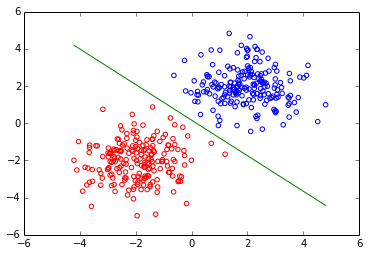
\includegraphics[scale=0.5]{stdev1_train_lam_0.png}
 \label{stdev1_train_lam_0}
 \caption{$\lambda = 0$, stdev1 train dataset}
 \end{figure}

\begin{figure}
 \centering
 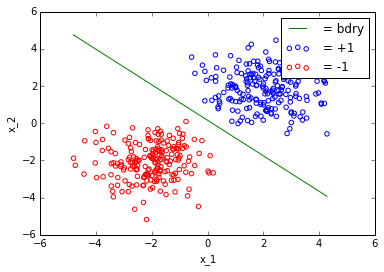
\includegraphics[scale=0.5]{stdev1_val_lam_0.png}
 \label{stdev1_val_lam_0}
 \caption{$\lambda = 0$, stdev1 validation dataset}
 \end{figure}
 % \quad
 % \subfloat[Run 2]{%
 % 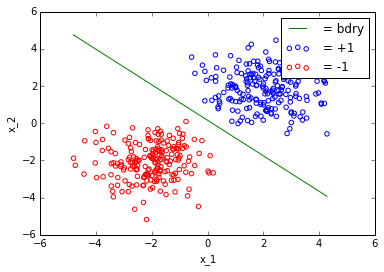
\includegraphics[scale=0.5]{stdev1_val_lam_0.png}
 % \label{stdev1_val_lam_0}
 % }
 % \caption{Results of logistic regression with $\lambda = 0$ for the training and validation sets.}
 % \end{figure} 

The other datasets (other than stdev1) are not linearly separable. Hence we don't have the ``weights running off to infinity'' problem that we had with stdev1. Since the stdev of the points in these datasets is larger (making them non-separable) we also expect the classfication error rate to be larger as well. The results for the stdev4 dataset are shown in Figures \ref{stdev4_train_lam_0} and \ref{stdev4_val_lam_0}. The classifier still exihibits relatively good performance in separating the data. Even though the data is noisy, the decision boundary is very similar to the one in the less noisy case, the stdev1 data.
\begin{figure}
 \centering
 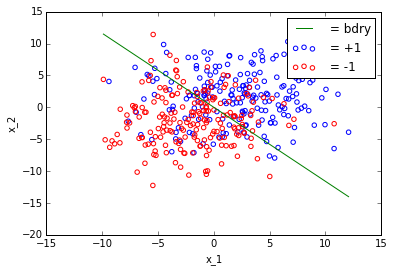
\includegraphics[scale=0.5]{stdev4_train_lam_0.png}
 \label{stdev4_train_lam_0}
 \caption{$\lambda = 0$, stdev4 train dataset}
 \end{figure}

\begin{figure}
 \centering
 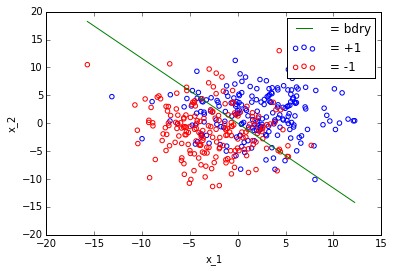
\includegraphics[scale=0.5]{stdev4_val_lam_0.png}
 \label{stdev4_val_lam_0}
 \caption{$\lambda = 0$, stdev4 validation dataset}
 \end{figure}
 %
 %
 In contrast the performance on the nonseparable dataset is quite poor. This makese sense since the data is not linearly separable.
\begin{figure}
 \centering
 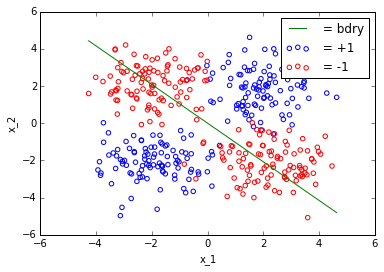
\includegraphics[scale=0.5]{nonsep_train_lam_0.png}
 \label{nonsep_train_lam_0}
 \caption{$\lambda = 0$, nonsep train dataset}
 \end{figure}

 Interestingly, even with the regularizer $\lambda$ set to $0$ the performance across the training and validation sets for a given dataset (e.g. stdev2) are comparable. This can be seen by the similar missclassification rates across corresponding training and validation sets in Table \ref{lam_0}. This means that our logistic regression classifier is generalizing fairly well.


\subsection{$\lambda > 0$}
Now we analyze the results for different values of the regularizer $\lambda$. Figures \ref{nonsep_train_lam_10}, \ref{nonsep_train_lam_100}, \ref{nonsep_train_lam_1000} shows the result of running logistic regression on the nonsep dataset for different values of $\lambda$. The thing to note is that for different values of $\lambda$ the actual decision boundary, plotted in green, looks very similar. In fact what seems to be happening is that as $\lambda$ increases the optimal weight $w(\lambda)$ are just scaled down to zero. In fact if we define $\overline{w}(\lambda) = \frac{w(\lambda)}{||w(\lambda)||}$ then $\overline{w}(\lambda)$ is very similar across different values of $\lambda$. Thus the regularizer $\lambda$ is forcing the weights toward zero, i.e. $||w(\lambda)||$ is decreasing in $\lambda$, but the scaled weights $\overline{w}(\lambda)$ are staying essentially the same. This explains why the decision boundaries look the same across the three plots in Figure \todo{include reference} since $w_0 + w_1 x_1 + w_2 x_2 = 0$ and $c w_0 + c w_1 x_1 + c w_2 x_2 = 0$ (where $c > 0$ is a constant) define the same hyperplane. Thus in this case the regularizer $\lambda$ just serves to drive the weights toward zero, but does so in a way that doesn't significantly affect the classification boundary. Table \ref{w_lam_norm} shows how $||\tilde{w}(\lambda)|| \to 0$ as we increase $\lambda$.

\begin{table}[H]
\begin{tabular}{|c|c|}
\hline
$\lambda$ & $||\tilde{w}(\lambda)||$\\ \hline
$0$ & $0.034$ \\ \hline
$10$ & $0.0329$ \\ \hline
$100$ & $0.0242$ \\ \hline
$1000$ & $0.00067$ \\ \hline
\end{tabular}
\label{w_lam_norm}
\caption{Norm of $\tilde{w}(\lambda)$ for different values of $\lambda$ on nonsep train dataset.}
\end{table}

\begin{figure}
 \centering
 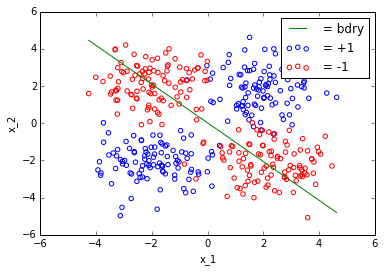
\includegraphics[scale=0.5]{nonsep_train_lam_10.png}
 \label{nonsep_train_lam_10}
 \caption{$\lambda = 10$, nonsep train dataset}
 \end{figure}
 \begin{figure}
 \centering
 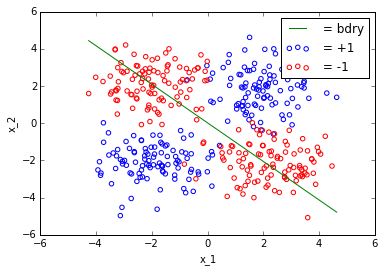
\includegraphics[scale=0.5]{nonsep_train_lam_100.png}
 \label{nonsep_train_lam_100}
 \caption{$\lambda = 100$, nonsep train dataset}
 \end{figure}
 \begin{figure}
 \centering
 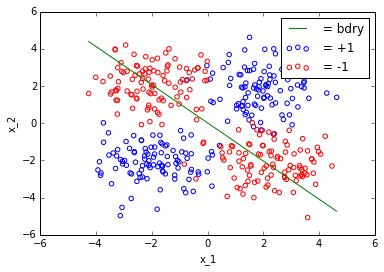
\includegraphics[scale=0.5]{nonsep_train_lam_1000.png}
 \label{nonsep_train_lam_1000}
 \caption{$\lambda = 1000$, nonsep train dataset}
 \end{figure}

For the nonseparable data the results look fairly identical. Not sure if we should expect something different . . . 


\section*{Titanic}

\begin{enumerate}
\item We perform ``interval'' type feature rescaling. Namely we rescale all the features so that they lie in $[0,1]$. The performance is shown in Figure \ref{titanic_logit}. Performing model selection leads us to choose $\lambda = 2.5$.
 \begin{figure}
 \centering
 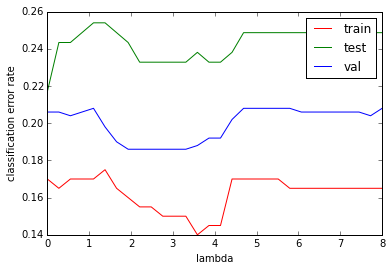
\includegraphics[scale=0.5]{titanic_logit.png}
 \label{titanic_logit}
 \caption{Results of logistic regression classifier on Titanic dataset for different value of $\lambda$.}
 \end{figure}

 \item 

 \item The classifiers (resulting from model selection in parts 1 and 2) for logistic regression (LR) and SVM are detailed in Table \ref{weights}. For LR we see that the most important features are which class you are in, your sex, and your age. Sex is by far the most important of those.
 %
 \begin{table}[H]
 \begin{tabular}{|c|c|c|}
 \hline
 Meaning & LR & SVM \\ \hline
 $w_0$ & $-0.854$ & \\ \hline
 1st Class & $0.35$ & \\ \hline
 2nd Class & $0.33$ & \\ \hline
 3rd Class & $-0.69$ & \\ \hline
 Sex  & $1.65$ & \\ \hline
 Age & $-0.267$ & \\ \hline
 \# Siblings/Spouses & $-0.004$ & \\ \hline
 \# Parents/Children & $0.23$ & \\ \hline
 Fare & $0.16$ & \\ \hline
 Southampton & $-0.255$ & \\ \hline
 Cherbourg & $0.23$ & \\ \hline
 Queenstown & $0.026$ & \\ \hline
 \end{tabular}
 \caption{Classification weights}
 \label{weights}
 \end{table}


\end{enumerate}

\end{document} 


% This document was modified from the file originally made available by
% Pat Langley and Andrea Danyluk for ICML-2K. This version was
% created by Lise Getoor and Tobias Scheffer, it was slightly modified  
% from the 2010 version by Thorsten Joachims & Johannes Fuernkranz, 
% slightly modified from the 2009 version by Kiri Wagstaff and 
% Sam Roweis's 2008 version, which is slightly modified from 
% Prasad Tadepalli's 2007 version which is a lightly 
% changed version of the previous year's version by Andrew Moore, 
% which was in turn edited from those of Kristian Kersting and 
% Codrina Lauth. Alex Smola contributed to the algorithmic style files.  
